\chapter{Vocal Accommodation for Conversation Intelligence}
\label{chap:conv_analysis}

\lettrine{C}{onversation} intelligence deals with the analysis and management of data accumulated during an interaction, e.g., to draw conclusion about the interlocutors.
This chapter includes examples of vocal accommodation used as a mean for analyzing patterns, structures, and behaviors in different interaction setups.

\pagebreak

\section{Conversation intelligence}
\label{sec:conversation_intelligence}

%\Acf{ci}, also known as \textit{conversation IQ} (\aca{ci}), is\ldots

\citet{Glaser2016conversational}
\citet{SilberVarod2018human}

\section{Speech variations in human-\acl{hci}}
\label{sec:speech_variations_in_hhci}

% *** Alexa ESSV paper ***

\section{abstract}

This paper presents a study that examines the difference of certain phonetic features between \ac{hds} and \ac{dds} in human-human-computer interactions.
The corpus used for the analyses consists of tasks performed by participants in cooperation with a human confederate and/or a computer-based interlocutor.
This includes distributional and temporal analyses, examining the similarities and differences of the overall distribution of the measured features and time-based changes throughout the interactions. 
The features \acl{f0}, intensity, and \acl{ar} were selected for analysis.
Results show significant differences in a majority of the cases for two of the three selected features as well as insights regarding the participants' speech behavior during the interaction.
These outcomes provide a look into further aspects of \ac{hds} and \ac{dds} and speech-related features in conversation analysis, which may help studies in topics like addressee detection or \ac{hci}.

\section{Introduction}
\label{sec:introduction}

Nowadays, we are witnessing in our everyday lives an ever-growing presence of devices with spoken interaction capabilities, like \acp{pa}, speech-activated cars, hands-free medical assistants, and \acp{its}, to name a few.
The question arises, therefore, whether different speech patterns and characteristics emerge in such \ac{hci} than in \ac{hhi}; and if yes, which.

It has been demonstrated that humans may change their speech behavior when interacting with computer-based systems.
One way of measuring such changes is in terms of linguistic similarity between the interlocutors.
In various \ac{hci} experiments, participants have been shown to speak differently to computers in general, and also change their speech during the interaction (see \citet{Branigan2010linguistic}, for examples).
However, these are human-computer interactions  that emphasize the comparison between different configurations of the system itself \citep[e.g.,][]{Levitan2016implementing}.
Moreover, no direct comparison between human-directed and computer-directed speech was performed.

In this paper, we present conversation-level analyses of speech changes in human-human-computer interactions with an Amazon Alexa device (Echo Dot, 2nd generation) as the computer-based interlocutor.
We chose to analyze three phonetic features: \ac{f0}, intensity, and \ac{ar}.
These analyses show the differences in the human interlocutor's behavior when addressing the confederate human speaker or the computer interlocutor.
Examples of distributional and temporal changes across the interaction are given.
These analyses are performed on the \acf{vacc}~\citep{Siegert2018VACC}, which comprises two experimental scenarios: the Calendar Module (formal interaction) and the Quiz Module (informal interaction).

Other studies, like \citet{Shriberg2013addressee} and \citet{vanTurnhout2005identifying}, used similar corpora to study automatic addressee detection.
The present work does not set detection and classification as its goal, but rather aims to provide insights and measures that might be useful for such tasks.
The results of the analyses show that the differences between the distributions for the features \ac{f0} and intensity in \ac{hds} and \ac{dds} contexts were significant in \SI{74}{\percent} and \SI{89}{\percent} of the cases, respectively, while for \ac{ar} in only \SI{13}{\percent}.
This sheds light on the similarities and differences in speech when addressing humans and computers.

\section{Dataset}
\label{sec:dataset}

The \ac{vacc} \citep{Siegert2018VACC} was utilized to examine differences in \ac{hds} and \ac{dds}.
This corpus consists of conversations between one or two human interlocutors with the 2nd generation of the commercial smart speaker Amazon Echo Dot, which uses the skills and voice of the virtual assistant Alexa.
The conversations comprise a formal and an informal scenario conducted either with the participant alone or together with a confederate accompanying person, which allows investigating how humans address computer-based systems.

% a formal and an informal one, are designed. The scenarios are conducted by the participants alone and with an accompanying person. Furthermore, questionnaires are used to get a self-evaluation of the participants in terms of their experience of the interaction and their conscious changes in voice  and behaviour while addressing a technical system. Additionally, also their experience with technical systems and the evaluation of the utilized commercial voice assistant is retrieved via questionnaires. The corpus consists of high-quality microphone recordings of 27 German speaking subjects, all students at the University Magdeburg.

%\begin{table}[t]
%	\caption{Summary of the \acs{vacc} metadata}
%	\label{tab:dataset_metadata}
%	\begin{center}
%		\begin{tabular}{l@{\hspace{2cm}}l}
%			\toprule
%			Language 					& German												  \\
%			\#Participants			 	& 27 (14 female / 13 male)								  \\
%			Age mean	 				& Mean 24 $\pm$ 3.32 years								  \\ %Min: 20; Max: 32
%			\#Interactions				& 108												   	  \\
%			Total time			 		& \SI{17}{\hour} \SI{7}{\minute} (mean: \SI{31}{\minute}) \\
%			Total number of utterances	& $~\sim$13,500											  \\
%			\bottomrule
%		\end{tabular}
%	\end{center}
%\end{table}

\subsection{Setting and participants}
\label{subsec:setting_and_participants}

\ac{vacc} contains recordings of 27 German native speaking students from Otto von Guericke University Magdeburg.
Each speaker participated in four recordings, for a total of 108 interactions (27 participants $\times$ 2 scenarios $\times$ 2 conditions).
The total recording time is \SI{17}{\hour} \SI{7}{\minute} (\SI{31}{\minute} on average per interaction) containing \num{\sim 13500} utterances.
The number of female (14) and male (13) participants is nearly equal, and their ages range from 20 to 32 years (mean~24.11; sd~3.32).
The participants came from different study programs, including computer science, engineering, humanities, and medical sciences.
Thus, this dataset is not biased towards students with stronger technical background.

An experiment with a participant consists of four interactions:
A formal and an informal scenario, each carried out in solo and confederate conditions.
An interaction was finished either by reaching its aim or by stopping it to avoid participant frustration in case no further progress could be made.

In the first scenario, the Calendar Module, each participant was asked to make appointments with a project partner.
The participant's calendar was stored online and was only accessible via Alexa's voice commands.
In the solo condition, the participants only received written information about the confederate's available dates and had to interact with Alexa on their own.
In the confederate condition, the confederate provided the relevant information.
Therefore, the participant had to interact with both Alexa and the confederate to find available time slots for the appointments.

In the second scenario, the Quiz Module, the participant answered trivia questions like \enquote{When was Albert Einstein born?}, which are mostly assumed to be too difficult to answer correctly without Alexa's help.
In the solo condition, the participants had to find the correct strategy for formulating questions for Alexa on their own own, whereas in the confederate condition the participant and the confederate teamed up to decide on a strategy. 

\subsection{Annotations}
\label{subsec:annotations}

Each utterance in an interaction was annotated with its speaker, context, and textual transcription.
The speaker of each utterance could be the participant, Alexa, or the confederate.
The context marked the type of interaction of the utterance, which include \ac{hds}, \ac{dds}, cross-talk, off-talk, laughter, and more.
To deal with clearer data, only \ac{hds} and \ac{dds} contexts were used for analysis in this paper (see \cref{sec:method}).
The transcription was obtained using the Google Cloud Speech API automatic speech recognition service.

\section{Method}
\label{sec:method}

To make the comparison between \ac{hds} and \ac{dds} more direct, we selected only those interactions where the participants talked with both the device and the confederate.
The remaining \SI{50}{\percent} of the dataset includes one calendar task and one quiz task for each of the 27 participants.
This subset was analyzed based on the audio signals of the interactions only.
The turn annotations were used to determine to which of the three speakers the measured values should be ascribed.
The text transcription was not utilized for this study.

Each interaction was analyzed using the audio from the participant's microphone (where both the confederate and the device are audible as well) and the annotations described in \cref{subsec:annotations}.
To increase temporal resolution, the audio signals were cut into two-seconds slices.
A single slice always contains audio from a turn of a single speaker, any remainder shorter than \si{2} seconds gets a slice of its own.
For example, a turn of \SI{5.2}{\second} in length was sliced into three slices of \SI{2}{\second}, \SI{2}{\second}, and \SI{1.2}{\second}.
Each of the features was then analyzed within a single slice.

The following phonetic features were analyzed:\\
\textbf{\Acf{f0}} -- the mean pitch measured within the audio slice with automatic time step selection and a range between \SIlist{60;350}{\hertz}.\\
\textbf{Intensity} -- the mean intensity measured within the audio slice with automatic time step selection.\\
\textbf{\Acf{ar}} -- the ratio of number of syllables to phonation time within the audio slice, as described in \citet{DeJong2009arcitulcationrate}.\\
All features were measured using Praat\footnote{version 6.0.35} \citep{Boersma2001praat} scripts that processed the signal of the participant's microphone.
To filter out noise and concentrate on the more characteristic speech style, only values between the first and third quartiles were taken into account for the non time-based analyses.
Furthermore, turns not annotated as \ac{hds} or \ac{dds} (e.g., cross-talk or off-talk) were also ignored.

\section{Results}
\label{sec:results}

As a first measure of speech characteristics, the means, medians, and \aclp{sd} of the selected features in the participants' speech in each of the interactions were calculated in \ac{hds} and \ac{dds}.
The absolute values reflected in the means and medians can shed light on the overall range of values used with each of the two interlocutors,
for example, due to different gender (Alexa was always set with a female voice and the confederate was always male) or assumed comprehension capabilities of humans and computers.
The \aclp{sd} show the variability of a feature with each interlocutor, which may indicate a different production style.

Each target feature was measured and listed chronologically throughout the interaction.
These lists were divided into four distributions based on speaker and context: participant talking to the confederate, participant talking to Alexa, confederate talking to participant, and Alexa talking to participant.
The contrast between \ac{hds} and \ac{dds} is observable within the participant's speech only, which was active in both contexts.
The significance level of the difference between these two distributions was measured using a two sample t-test with $\alpha=0.05$.

\cref{fig:hds_dds_dist_pitch_comparison} shows examples of the distributions of the participant's \ac{f0} in \ac{hds} and \ac{dds} contexts.
Since the device always used the default Alexa female voice and the confederate was always male, there is a natural gap between their \ac{f0}.
This gap leaves room for convergence to occur, i.e., when two interlocutors become more similar to each other over time with respect to some measured feature.
In \SI{74}{\percent} of the cases out of the 54 analyzed interactions the difference of means of the participant's \ac{hds} and \ac{dds} \ac{f0} distributions was significant.
In \SI{85}{\percent} of the cases where the difference was significant, more of the probability mass of \ac{dds}'s distribution contained higher values than \ac{hds}'s, and therefore more similar to Alexa.

\begin{figure}[t]
	\centering
	\subfigure
	[An example of \ac{hds} and \ac{dds} distribution densities with a \emph{significant} difference (p-value$\ll$0.0001, $\alpha=0.05$) extracted from the \ac{f0} measures of participant 20171127A in the Quiz task.]
	{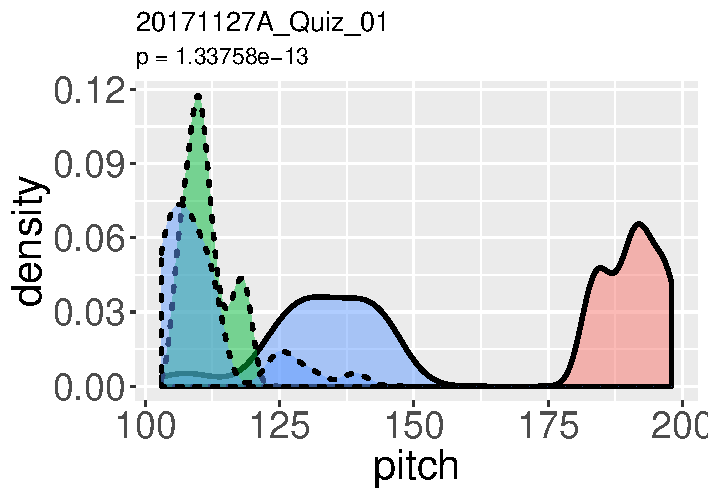
\includegraphics[width=0.45\textwidth]{20171127A_Quiz_01_pitch_dist}
		\label{fig:hds_dds_dist_signif}} 
	\hfill % no empty line here to avoid staring a new paragraph (figures will be vertically aligned)
	\subfigure
	[An example of \ac{hds} and \ac{dds} distribution densities with a \emph{non-significant} difference (p-value=0.71, $\alpha=0.05$) extracted from the \ac{f0} measures of participant 20171127C in the Calendar task.]
	{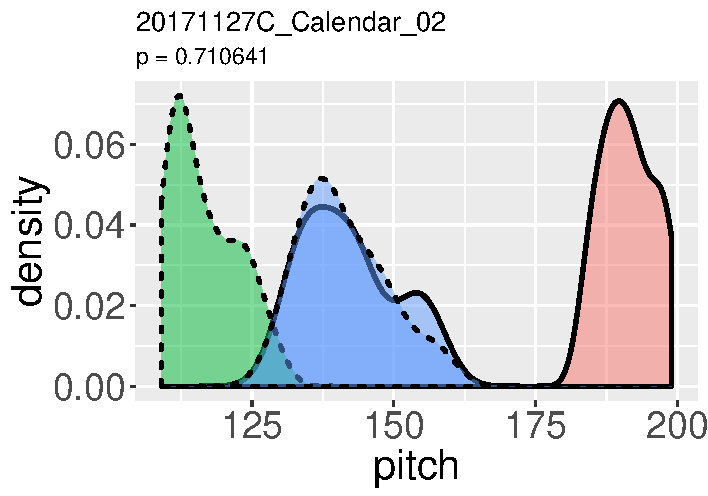
\includegraphics[width=0.45\textwidth]{20171127C_Calendar_02_pitch_dist}
		\label{fig:hds_dds_dist_nonsignif}}
	\caption
	[Distribution densities of f$_0$ in human-directed and device-directed speech]
	{A \emph{significant} \subref{fig:hds_dds_dist_signif} and a \emph{non-significant} \subref{fig:hds_dds_dist_nonsignif} difference between distribution densities of participants' \ac{hds} and \ac{dds} \ac{f0}.
		The colors represent distributions of Alexa (red), the confederate (green), and the participant (blue).
		The line style differentiates between \ac{hds} context (dashed line) and \ac{dds} context (solid line).}
	\label{fig:hds_dds_dist_pitch_comparison}
\end{figure}

\cref{fig:hds_dds_violin_intensity_comparison} shows examples of the distributions of the participant's intensity in \ac{hds} and \ac{dds} contexts.
Unlike in the case of \ac{f0}, absolute measured values may not be as meaningful due to the device's and the confederate's location relative to the participant's microphone.
As explained in \cref{sec:method}, the signal from the participant's microphone was used for the difference analyses.
This means that the absolute values of the participant's intensity  in \ac{hds} and \ac{dds} can be compared directly, but only indirectly with Alexa's and the confederate's.
Therefore, in \cref{fig:hds_dds_violin_intensity_comparison} the differences in distribution and frequency can be compared within a context, but the values should only be compared within the participant's speech (in blue).
In \SI{89}{\percent} of the cases out of the 54 analyzed interactions the difference of means of the participant's \ac{hds} and \ac{dds} intensity distributions was significant.
Moreover, participants tended to speak to Alexa with a louder voice than to the confederate.

\begin{figure}[t]
	\centering
	\subfigure
	[An example of \ac{hds} and \ac{dds} values with a \emph{significant} difference (p-value$\ll$0.0001, $\alpha=0.05$) extracted from the intensity measures of participant 20171127A in the Quiz task.]
	{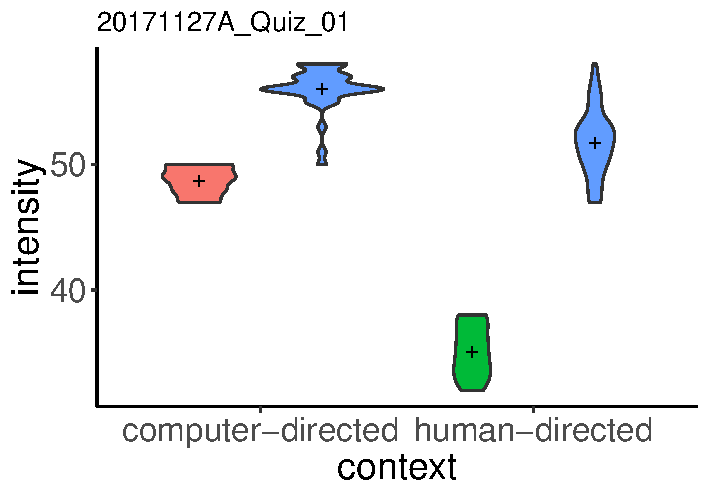
\includegraphics[width=0.47\textwidth]{20171127A_Quiz_01_intensity_violin}
		\label{fig:hds_dds_violin_signif}} 
	\hfill % no empty line here to avoid staring a new paragraph (figures will be vertically aligned)
	\subfigure
	[An example of \ac{hds} and \ac{dds} values with a \emph{significant} difference (p-value=0.55, $\alpha=0.05$) extracted from the intensity measures of participant 20171127C in the Calendar task.]
	{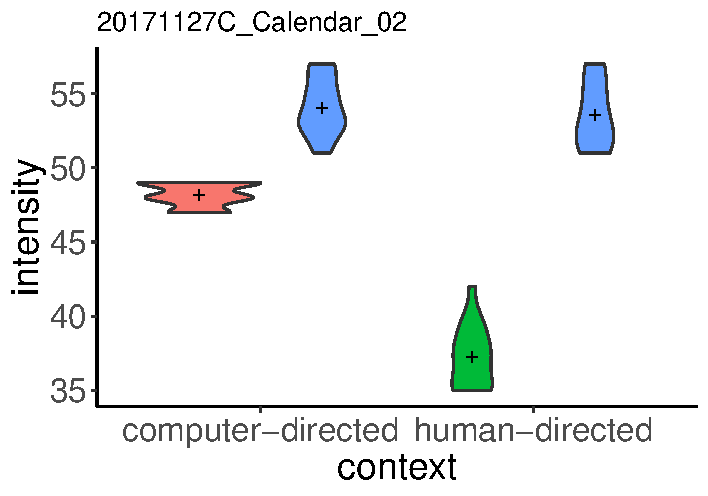
\includegraphics[width=0.47\textwidth]{20171127C_Calendar_02_intensity_violin}
		\label{fig:hds_dds_violin_nonsignif}}
	\caption
	[Distribution densities of intensity in human-directed and device-directed speech]
	{A significant \subref{fig:hds_dds_violin_signif} and non-significant \subref{fig:hds_dds_violin_nonsignif} difference between extracted values of participants' \ac{hds} and \ac{dds} intensity.
		The colors represent distributions of Alexa (red), the confederate (green), and the participant (blue).
		\ac{hds} is plotted in the right, and \ac{dds} in the left of the plot.
		The width of the box represents the frequency of the values and the \enquote*{+} sign marks their respective means.}
	\label{fig:hds_dds_violin_intensity_comparison}
\end{figure}

The differences of \acf{ar} distributions in \ac{hds} and \ac{dds} were calculated as well.
In \SI{13}{\percent} of the cases out of the 54 analyzed interactions the difference of means of the participant's \ac{hds} and \ac{dds} \ac{ar} distributions was significant.
This shows that the participants largely spoke at the same speed with the confederate and the device.
It was found that the articulation rate was lower in some specific cases where the participant tried to improve her/his intelligibility to the system, specifically when the system's output indicated that it could not understand the participant's utterance.
While such utterance-level changes are interesting and may point to a temporary change in behavior, a more detailed analysis is outside the scope of this study, which concentrates on interaction-level behavior.

Looking at the distribution differences of the selected features in \ac{hds} and \ac{dds} sheds light on the general speech behavior in these contexts.
However, this analysis leaves out an important aspect of spoken interaction, namely the time dimension.
While the static measures of distributions show the overall range and frequency of the values, temporal analysis adds the information as to how they changed over time.
Adding the time dimension gives an overview of the interaction's structure and reveals fine-grained information regarding its characteristics, such as turn lengths, turn switching, pauses, density of a speaker's utterances, convergence or divergence effects, etc.
For example, \cref{fig:hds_dds_time_pitch} shows a case where the the absolute \ac{f0} values are roughly the same in \ac{hds} and \ac{dds}, namely around \SI{150}{\hertz}, but the behavior of the participant is different.
In the \ac{dds} context, the participant generally keeps a stable distance from Alexa's voice, whereas in the \ac{hds} context the \ac{f0} values are closer to the confederate.
In both contexts, the participant's \ac{f0} starts around \SI{150}{\hertz}.
However, in \ac{hds} the minimum \ac{f0} is only slightly below this initial value, whereas in \ac{dds} it drops as far as \SI{25}{\hertz} lower.
An example for the intensity feature is shown in \cref{fig:hds_dds_time_intensity}.
Unlike the previous example, here the absolute values steadily differ by about \SI{5}{\decibel}, but the overall change is similar.
That is, in both cases the intensity rises from the beginning to around a quarter of the interaction's duration, and then decreases again until the end (in \ac{hds} more quickly than in \ac{dds}) down to approximately the same value as at the beginning.

Since \cref{fig:hds_dds_time_comparisons} shows two examples of the Quiz task performed by two different participants, it is possible to compare the structure of these interactions as well.
As described in \cref{sec:dataset}, the Quiz task in the confederate condition is designed so that the two human speakers needs to find an effective way to solve the questions using Alexa.
After improving their strategy, the lead should ultimately be taken by the participant, who interacts with Alexa to solve the questions as quickly and correctly as possible.
In both examples, the interaction starts with relatively short turns and rapid context changes.
This might be ascribed to the fact that the participant is still trying to figure out the best way to interact with Alexa and the confederate.
Then, sometime after the middle of the interaction, there is a larger block of \ac{dds} only, followed by some more turns of \ac{hds}.
Finally, the interactions end with another, shorter, block of \ac{dds}, in which the participants finish the last questions of the quiz.
This structure was found to be typical for the Quiz task.

\begin{figure}[t]
	\centering
	\subfigure
	%	[An example of \ac{f0} changes over the time of the interaction.
	%	In \ac{dds}, the speaker starts a bit above \SI{150}{\hertz} and ends slighly beneath it, generally maintaining the distance from the device's values.
	%	In \ac{hds}, the contour starts around the same value as in \ac{dds}, but gradually goes down towards the confederate and then up again, staying in the same range of values as the human speaker.
	%	This shows a different behavior with similar values.]
	{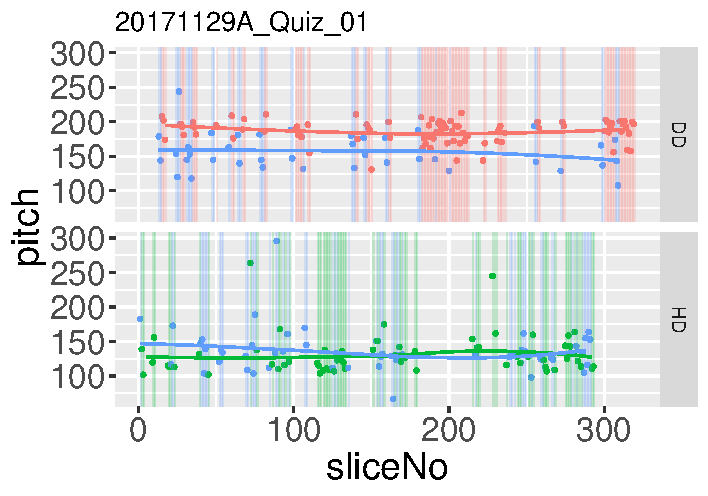
\includegraphics[width=0.49\textwidth]{20171129A_Quiz_01_pitch_time}
		\label{fig:hds_dds_time_pitch}} 
	\hfill % no empty line here to avoid staring a new paragraph (figures will be vertically aligned)
	%	\subfigure
	%	[An example of intensity changes over the time of the interaction.
	%	In both \ac{hds} and \ac{dds} contexts, there are a rise and a fall around the same time in the participant's values.
	%	However, the absolute values differ.
	%	This shows a similar behavior with different values.]
	{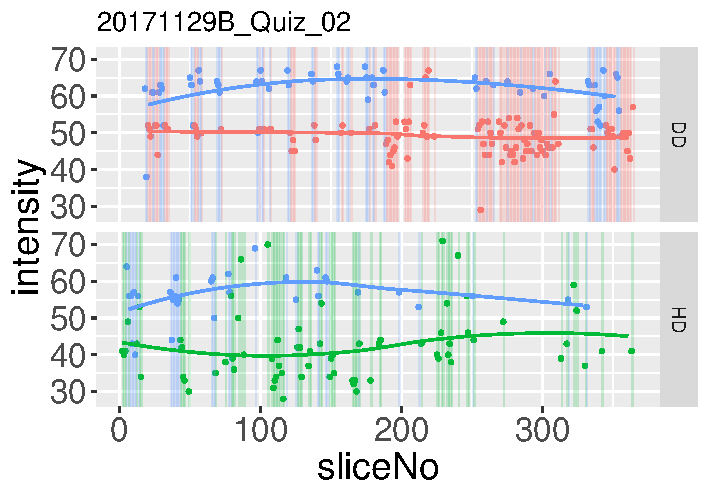
\includegraphics[width=0.49\textwidth]{20171129B_Quiz_02_intensity_time}
		\label{fig:hds_dds_time_intensity}}
	\caption
	[Temporal f$_0$ trends comparison of \acs{hhi} and \acs{hci} turns]
	{The changes in pitch (left) and intensity (right) over time in \ac{dds} (upper part) and \ac{hds} (lower part).
		The time spans on the x-axis are represented by turn slices, as explained in \cref{sec:method}, and the y-axis shows the value of the feature.
		A slice's background color indicates the speaker in this slice and the circle with the same color, the measured value of the feature in it.
		Alexa's voice is shown in red, the confederate in green, and the participant in blue.
		The lines are smoothed values calculated by LOESS \citep{Cleveland1988locally}.}
	\label{fig:hds_dds_time_comparisons}
\end{figure}

\cref{tab:results_summary} summarizes the results.

\section{Discussion}
\label{sec:discussion}

\cref{sec:results} presented the results for the features \ac{f0}, intensity, and \acf{ar}.
The first two show a greater degree of difference between \ac{hds} and \ac{dds}, and the latter, a smaller one.
One possible explanation for the different \ac{f0} distributions is the natural difference in male and female \ac{f0} (Alexa used a female voice while the confederate was always male) and the fact that humans sometimes tend to match their \ac{f0} to the interlocutor.
In that case, the results shown here point to the fact that the participants generally treated Alexa as a human interlocutor with regards to \ac{f0} behavior, as opposed to, for example, matching only the human interlocutor and talking to the computer-based interlocutor using the same \ac{f0}.
A similar effect was found for intensity.
Since the device and the confederate were spaced approximately at the same distance from the participants, there was no apparent reason for the participants to speak more loudly with either interlocutor.
Therefore, an explanation of the tendency to speak more loudly to the device may come from the intuition that a computer-based system has a harder time to understand human speech and therefore needs a clearer signal.
Another explanation may be the illusion that Alexa feels more distant than the human interlocutor, because Alexa is not an embodied agent.
Keeping in mind that an interaction aims to be as efficient as possible using minimum amount of energy, it seems like changing these features helped -- or at least felt like helping -- the participant to interact more efficiently with the device.
This is not the case with \ac{ar}, which shows a lower degree of differences.
Slower, more carefully articulated speech, occurs less often in regular speech than louder speech or higher pitch.
Such enhanced articulation not only takes longer to produce, but also requires more effort, making it a less preferred way to communicate, unless it is necessary.
In a somewhat formal, experimental setting, participants are likely to speak more slowly than usual, and the motivation to complete the task in a short time does not encourage them to speak even more slowly.
This supports the hypothesis that extra slow speech would only be used when necessary, e.g., when a repetition is required due to a misunderstanding of an utterance.
Even in that case, the overall \ac{ar} tends to increase afterwards, to make the interaction more fluent again.

Future work may go in two main directions, both concerning a temporal aspect of interaction.
The first has do to with analysis on the speech signal level, where the changes in measures over time can capture phenomena like convergence or divergence.
In a more comprehensive analysis in this direction, more detailed patterns may emerge.
Such an analysis can concentrate on one context or on comparing patterns in both \ac{hds} and \ac{dds}.
Additionally, more features can be measured to reveal more details regarding speech behavior.
The second potential direction may highlight behavioral patterns of the conversation and turn levels.
This can include a closer examination of the interaction structure as a whole, the dynamics of turn changes, pauses and repetitions, etc.
Such an analysis can be performed on interactions in solo and confederate condition to inspect whether humans deal with the same task differently with a computer alone, than when another human is involved.

\begin{table}[t]
	\centering
	\caption
		[Percentage of significantly different interactions]
		{Summary of results.
		The percentage of interactions in which the difference of distribution means was significant for each feature, and their mean and \acf{sd}.}
	\label{tab:results_summary}
	\begin{tabular}{lSSS}
		\toprule
		& \acs{f0} 						& {intensity}				& \acs{ar}									\\
		signif. diff.					& \SI{74}{\percent}			& \SI{89}{\percent}		& \SI{13}{\percent} \\
		\acs{hds} mean (\acs{sd}) 		& 10.5\,\si{\hertz}			& 2.95\,\si{\decibel}	& 0.627				\\
		\acs{dds} mean (\acs{sd}) 		& 10   \,\si{\hertz}		& 2.61\,\si{\decibel}	& 0.634				\\
		\bottomrule	
	\end{tabular}
\end{table}

\section{Conclusion}
\label{sec:conclusion}

In this paper, we presented an analysis of phonetic features in a study based on a subset of a human-human-computer corpus, which includes two tasks with 108 interactions in total.
Three interlocutors participate in the interactions: the participant, a confederate, and an Amazon Alexa device.
The features \ac{f0}, intensity, and \ac{ar} were analyzed for each of the three interlocutors across each interaction.
Based on the dataset's turn annotations, the utterances of the speakers were categorized as either \ac{hds} or \ac{dds} context.
First, the participant's speech in both contexts was examined by comparing the distributions of the measured values in each context.
Then, the difference of the distributions was checked for significance.
Finally, the temporal changes of the features across the interaction were examined as well.

The difference between the distributions was significant in \SI{74}{\percent} and \SI{89}{\percent} of the interactions for \ac{f0} and intensity, respectively, and in \SI{13}{\percent} for \ac{ar}.
As for the temporal analysis, different patterns of changes were observed, like cases where the participant accommodated to the human interlocutor but not the computer and cases where a similar behavior was observed in both contexts.

% *** Alexa Interspeech paper ***

\section{abstract}

This study examines how the presence of other speakers affects the interaction with a spoken dialogue system.
We analyze participants' speech regarding several phonetic features, viz., fundamental frequency, intensity, and articulation rate, in two conditions:
with and without additional speech input from a human confederate as a third interlocutor.
The comparison was made via tasks performed by participants using a commercial voice assistant under both conditions in alternation.
We compare the distributions of the features across the two conditions to investigate whether speakers behave differently when a confederate is involved.
Temporal analysis exposes continuous changes in the feature productions.
In particular, we measured overall accommodation between the participants and the system throughout the interactions.
Results show significant differences in a majority of cases for two of the three features, which are more pronounced in cases where the user first interacted with the device alone.
We also analyze factors such as the task performed, participant gender, and task order, providing additional insight into the participants' behavior.

\section{Introduction}
\label{sec:introduction}

In recent years, the market for commercial \acp{va} has rapidly grown.
For example, Microsoft Cortana had 133 million active users in 2016 \citep{Osborne2016why} and Echo Dot was Amazon's best-selling product between 2016 and 2018 \citep{Dickey2017echo}.
Furthermore, \SI{72}{\percent} of people who own a smart speaker say they often use their devices as part of their daily routine \citep{Kleinberg2018ways}.

The big advantage of \acp{va} is their simple operation.
Using nothing but speech commands, users can perform tasks like playing music, searching the web, shopping online, etc.
In the future, we are likely to witness an ever-growing presence of devices with spoken interaction capabilities, like speech-activated cars, hands-free medical assistants, and intelligent tutoring systems.
This will increase the demands on voice-activated devices even more, as they will need to support more functionalities in a way that is comfortable and intuitive for the users.
Additionally, it can be expected that such devices will be used not only by individuals, but also in more social contexts, i.e., where multiple humans are involved.
Therefore, we find it important to investigate not only \aclp{hci}, but also human-human-computer interactions.

Besides making the operation of such voice-activated systems simple and user-friendly, \acp{va} also aim to let users interact with them in a familiar, natural manner.
One property of natural interactions is the tendency to accommodate to the specific situation and interlocutors to  make the interactions more fluent and efficient \citep{Giles1991CAT,Gallois2015CAT}.
Linguistic accommodation is one aspect of this phenomenon, and it is found in various \ac{hhi} experiments \citep[e.g.,][]{Pardo2017phonetic,Schweitzer2017social}.
In various \ac{hci} experiments, it has been shown that participants speak differently to computers in general, and also change their speech behavior during the interaction, e.g., by \citet{Branigan2010linguistic} and \citet{Levitan2016implementing}.
However, these interactions include only the computer-based interlocutor and emphasize the comparison between different configurations of the system itself.
%Furthermore, these studies have never used an actual commercial \ac{va} system.
Moreover, they only examine the influence of the system's speech output on the user, but not the influence of other interlocutors.

The question tackled in this paper is whether and to what extent speaking to a second human interlocutor in addition to Alexa influences the accommodation in interaction with a \ac{va}.
More generally, we investigate whether users speak differently towards a computer-based system when another human participates in the interactions.
%To investigate this question and other factors, we utilize the \ac{vacc} \citep{Siegert2018VACC}, which comprises human-computer interactions of two different tasks, each of them performed once with the \ac{va} alone and once with the \ac{va} and a human confederate.
This was done using a set of interactions of participants with a \ac{va} alone or with a \ac{va} and a confederate.
Thus, it allows us to analyze the participants' accommodation to the \ac{va} in both social conditions.

% Empirical evidence of entrainment in human-human conversations has been documented for acoustic-prosodic features suchas intensity [7, 8, 9], speaking rate [2], and pitch [8, 9].
% Humans have been shown to entrain to their interlocutor’s languageat the lexical [10] or syntactic [11, 12] level, and on linguisticstyle [13, 14, 15].
% Motivated by Communication Accommoda-tion Theory (CAT) [16], which holds that speakers converge toor diverge from their interlocutors in order to attenuate or accen-tuate social differences, many studies have found links betweenentrainment and positive social behavior: entraining conversa-tional partners are perceived as more socially attractive, morecompetent, more likable, interactions with them as more suc-cessful, entrainment is positively correlated with learning gainsin automatic tutoring system and task success in Map Tasks[17, 18, 5, 3, 19, 1, 20, 21]

\section{Dataset}
\label{sec:dataset}

To analyze the influence of a confederate speaker in \ac{hci}, we used the \acf{vacc} \citep{Siegert2018VACC}.
This corpus comprises balanced human-computer (solo condition) and human-human-computer (confederate condition) interactions with a 2nd generation Amazon Echo Dot that uses the skills and female voice of the virtual assistant Alexa.
The first human speaker is the participant, which always takes part in the interactions.
The interactions consist of Calendar and Quiz tasks, where the former simulates a formal situation and the latter a rather informal situation.
This corpus, which alternately introduces a confederate speaker into otherwise similar conversations, allows investigating the influence of the confederate on the behavior of the participant.

\ac{vacc} contains recordings of 27 (14 female) German native speakers with a mean age of 24 years (sd 3.3).
Each participant performed the Quiz and Calendar tasks in both solo and confederate conditions, for a total of 108 interactions.
An interaction was finished either by completing the task or by stopping it prematurely in case no further progress could be made, to avoid participant frustration.
The latter, however, happened only a few times.
Approximately \num{13500} utterances were recorded, stretching over total recording time of \SI{17}{\hour} \SI{7}{\minute} (\SI{31}{\minute} on average per interaction).
The permutations of the tasks, conditions, and their order were balanced.

In the Calendar task, the participant made several appointments in pre-defined weeks with the confederate.
The participant's calendar was stored online, accessible only via Alexa.
In the solo condition, the participants got written information about the confederate's availability, whereas in the confederate condition, the confederate could be asked directly about it, resulting in a \emph{human-human-interaction}.
In the Quiz task, the participant answered trivia questions like, \enquote{When was Albert Einstein born?}
Although Alexa was not always able to immediately provide a full answer to all the questions, information could be incrementally gathered in multiple steps.
Here, the participant solved the quiz alone in the solo condition, or teamed up with the confederate so the two could discuss the question asking strategy.
The Quiz task was generally less formal than the Calendar task.
The confederate interacted only with the participant whenever he was involved.

The three interlocutors were arranged at an approximately equal distance from each other.
The two human speakers were seated and the Echo device was placed on a table.
More information about the recording setup and equipment is described by \citet{Siegert2018VACC}.
Turn times and speakers were manually annotated.

% \begin{figure}[!h]
% \begin{center}
% %\fbox{\parbox{6cm}{
% %This is a figure with a caption.}}
% %\includegraphics[scale=0.5]{image1.eps} 
% \includegraphics[width=0.75\linewidth]{figures/IMG_4798.jpg} 
% \caption{A snapshot of the data collection setup.The confederate speaker (left side) and the participant (right side) are sitting around a table, where the voice assistant (Amazon Alexa Echo Dot) is located.}
% \label{fig:wohnzimmer}
% \end{center}
% \end{figure}
% 
%	The recordings were conducted in a living room-like surrounding, see \cref{fig:wohnzimmer}.

% The aim of this setting was to enable the participant to get into a natural communication atmosphere (in contrast to the distraction of laboratory surroundings).
% The participant sat on the sofa (right side of the photo in Fig.~\ref{fig:wohnzimmer}) and interacted with the voice assistant system, placed on the table in the middle.
% The confederate speaker (present only in the two-person variants of each scenario) sat on the armchair (left side of the photo in Fig.~\ref{fig:wohnzimmer}).
% The positions were identical for all recordings of all participants to ensure comparability.

%Two high-quality neckband microphones (Sennheiser HSP 2-EW-3) were used to capture the voices of the participant and the confederate speaker.
%\todo{which one is used for the analyses?}
%Additionally a high-quality shotgun microphone (Sennheiser ME 66) captured the overall acoustics and the output of Amazon's Alexa.
%The recordings were stored in WAV format with \SI{44.1}{\kilo\hertz} sample rate and 16 bit resolution.
%The recordings were manually separated into utterances, which were additionally annotated with its speaker, context, and textual transcription.
%The speaker of each utterance could be the participant, Alexa, or the confederate.
%The context marked the type of interaction of the utterance, which include \ac{hds}, \ac{dds}, cross-talk, off-talk, laughter, and more.
%To deal with clearer data, only \ac{hds} and \ac{dds} contexts were used for analysis in this paper.
%The transcription was obtained using the Google Cloud Speech API automatic speech recognition service.
%\cref{tab:dataset_charact} summarizes the dataset characteristics.

%\begin{table}[t]
%	% \captionsetup{format=plain,justification=raggedleft,width=.4\textwidth,hangindent=0pt,skip=500pt}
%	\centering
%	\caption{\ac{vacc} dataset characteristics}
%	\label{tab:dataset_charact}
%	\begin{tabular}{L{3cm}L{3cm}}
%		\toprule
%	     Participants 				& 27														\\
%	     Sex 						& Male 13 / Female 14 										\\
%	     Total Recorded Data 		& \SI{17}{\hour} \SI{7}{\minute}							\\
%	     Experiment Duration 		& Mean: 31 min 												\\
%		  Age (years)				& Mean 24 (Std: 3.32)										\\	% Min: 20; Max: 32  \\
%	     Language 					& German													\\
%%	     Annotation 				& Transcription, Addressee, Laughter, Cross-Talk, Off-Talk	\\ 
%%	     Supplementary self-reports & Evaluation of interaction, AttrakDiff, Speaking style, Experiences in interacting with voice assistants\\
%		\bottomrule
%	\end{tabular}
%\end{table}

\section{Method}
\label{sec:method}

\begin{table}[t]
	\centering
	\caption
		[Percentage of significantly different interaction pairs]
		{Percentage of interaction pairs with significant differences with respect to each target feature with all the interactions together and separated by order tasks.}
	\label{tab:signif_conditions}
	\sisetup{table-format=3.0}
	\begin{tabularx}{\linewidth}{XSSS}
		\toprule
		\thead[l]{feature} & {\thead{any order}} & {\thead{solo first}}	& {\thead{confederate first}}	\\
		\midrule
		\acs{f0}	& 67	& 72	& 60 \\
		intensity 	& 67	& 76	& 56 \\
		\acs{ar}	& 30	& 31	& 28 \\
		\bottomrule	
	\end{tabularx}
\end{table}

All interactions from the \ac{vacc} were used for the analyses.
The comparisons were performed on pairs of interactions of the same task in the two conditions presented above.
%This puts the focus on the difference between those interactions in which the participant's speech may have been influenced by the confederate's speech and those where it could not be.
Only the audio signals of the interactions were used for analysis, as recorded by the headset microphone of the participant, which captured the speech of the confederate and Alexa as well.
Since the participants sat at an equal distance from Alexa and the confederate, this eliminates any spatial influence on their speech, e.g., in terms of intensity.
The turn annotations were used to determine to which of the three speakers the measured values belong.

To increase temporal resolution, the audio signals were split into two-second slices.
This duration is short enough to provide a decent temporal resolution shorter than a turn, but still long enough to calculate time-dependent features like \acf{ar}.
Splitting the turn also creates equal, consecutive, and more comparable time units for an interaction without introducing artificial boundaries by dividing it into a pre-defined number of parts \citep{Silber-Varod2018prosodic}.
This is especially important for the temporal analysis (\cref{subsec:temporal_analysis}).
Preliminary experiments with the corpus showed only very small changes in feature measurements with slices of longer duration.
The slicing was done per turn, so that a single slice contains the audio of a single speaker.
Any remainder of a turn duration got a slice of its own.

The following phonetic features were targeted, as they are in the focus of convergence research \citep{Levitan2011measuring,Natale1975Conv,Gregory1993Voice}:
\begin{description}[wide=0pt, leftmargin=0.5\parindent, nosep]
	\item[\Acf{f0}] mean pitch measured within the audio slice with automatic time step selection and a range between \SIlist{60;350}{\hertz}.
	\item[Intensity] mean intensity measured within the audio slice with automatic time step selection.
	\item[\Acf{ar}] ratio of number of syllables to phonation time within the audio slice, as described by \citet{DeJong2009arcitulcationrate}.
\end{description}

All features were measured in each slice individually using Praat\footnote{version 6.0.35} \citep{Boersma2001praat} scripts.
To filter out noise and concentrate on the more characteristic speech style, only values from the second and third quartiles were taken into account.
Furthermore, turns not annotated as speech for either of the speakers (e.g., cross-talk or off-talk) were also ignored.

\section{Results}
\label{sec:results}

\begin{figure}[t]
	\centering
	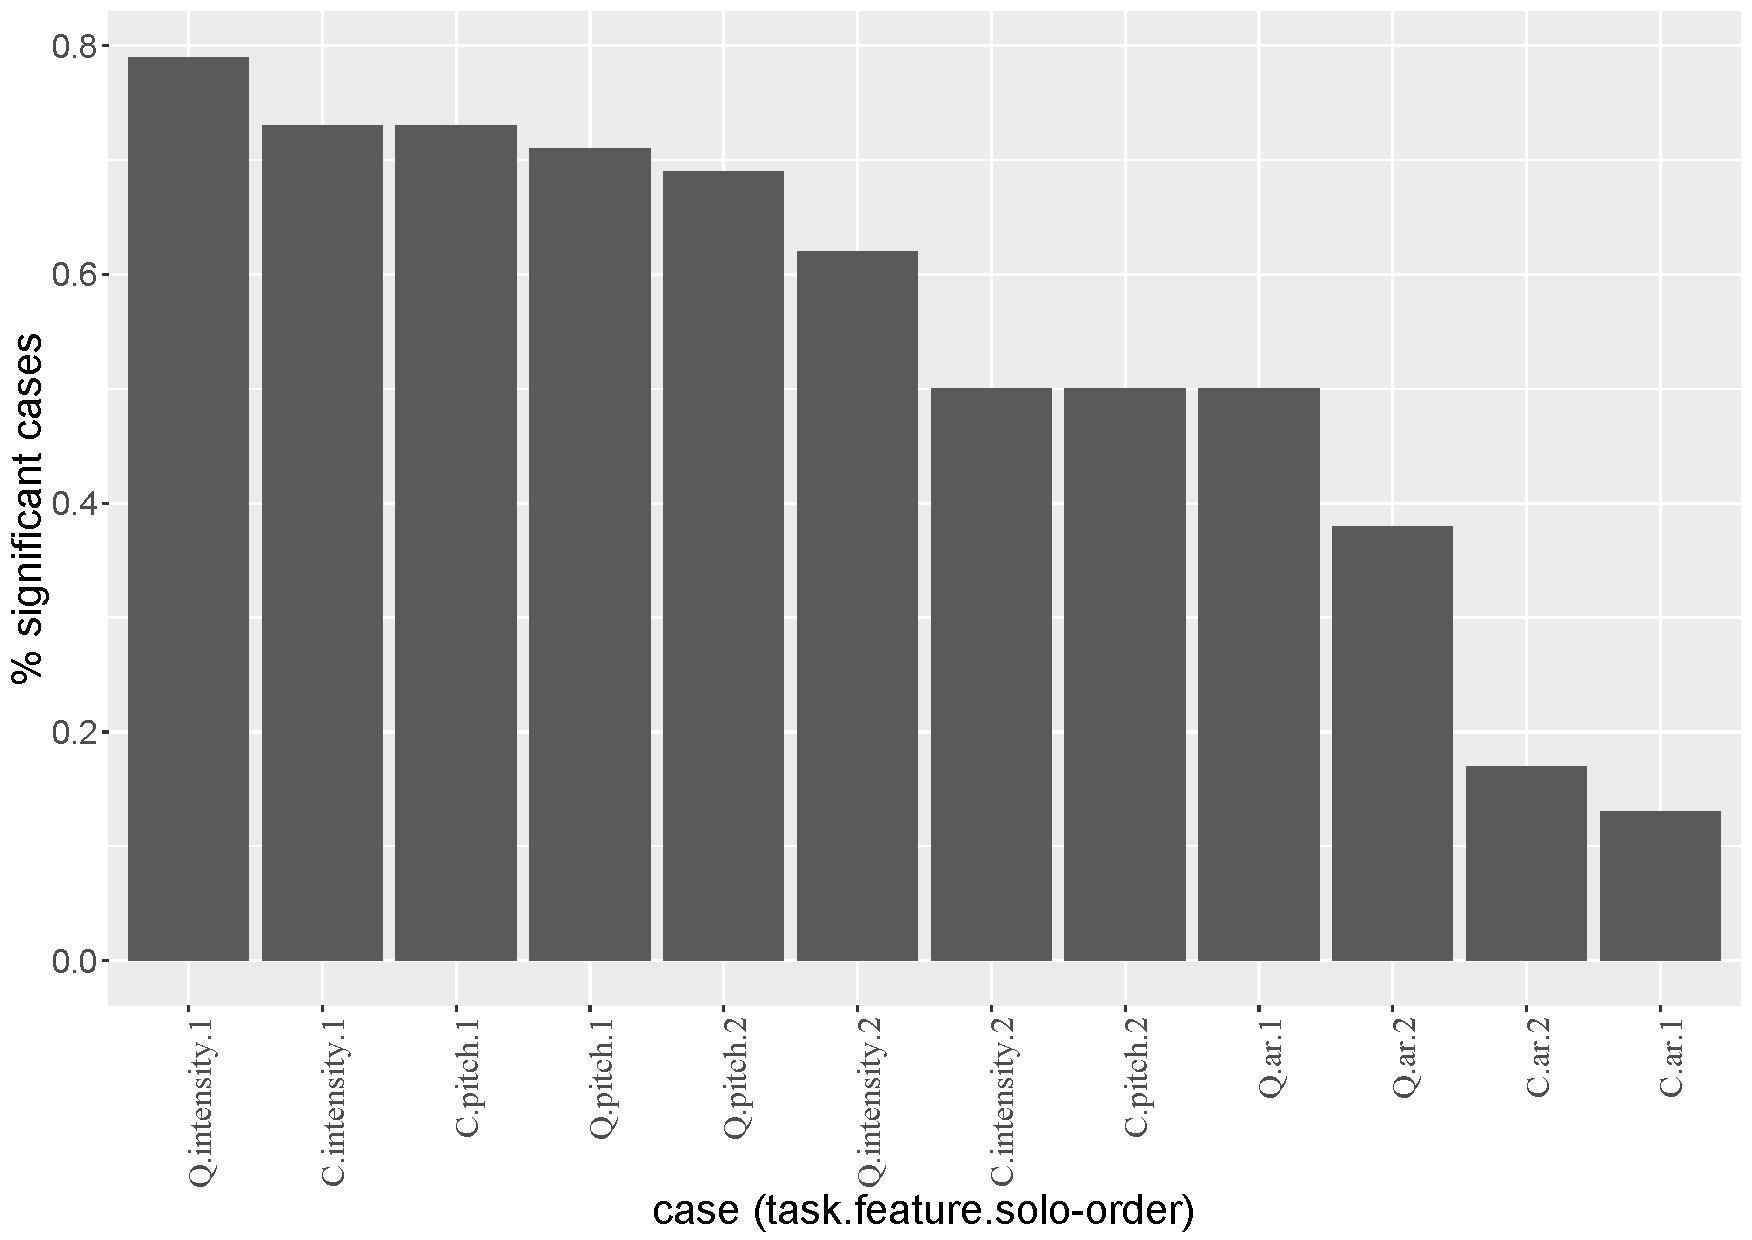
\includegraphics[width=\linewidth]{barplot_signif_cases}
	\caption
		[short caption]
		{Percentage of instances with a significant difference between solo and confederate conditions in each case.
		A case is a combination of the factors \emph{task}, \emph{feature}, and \emph{order}.
		For example, the case \emph{Q.intensity.2} contains the comparisons of intensity in interactions of the Quiz task where solo condition was performed second (and the confederate condition first).}
	\label{fig:signif_cases_ordered}
\end{figure}

Two separate analyses were carried out: distributional and temporal.
The first looks at global differences on the interaction level of the participant's and the computer-based interlocutor's productions between solo and confederate conditions.
It also checks whether the order in which the tasks were performed had any influence on the changes as well (see \cref{tab:signif_conditions,fig:signif_cases_ordered}).
The second examines time-based, continuous changes in the proximity between the participant's and the device's productions with emphasis on the \emph{condition} factor, and then also provides additional insights for the factors \emph{sex}, \emph{task}, and \emph{order} (\cref{fig:condition_convergence_comparison,fig:alluvial}).

\subsection{Distributional analysis}
\label{subsec:distributional_analysis}

\begin{figure*}[t]
	\centering
	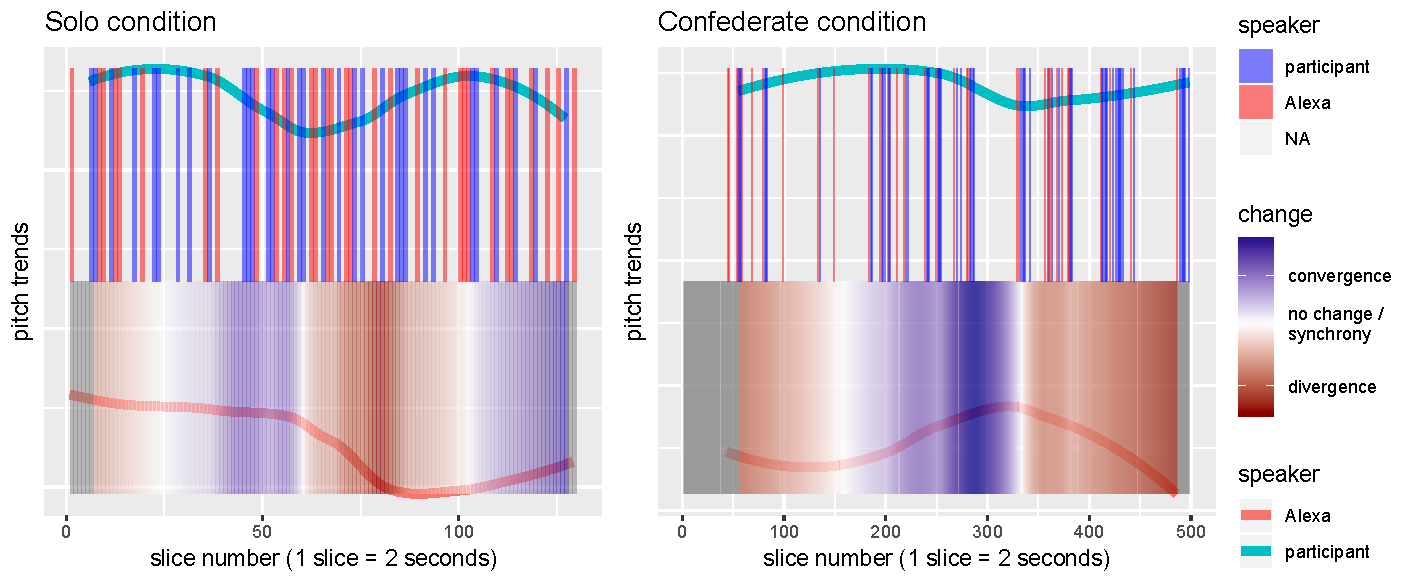
\includegraphics[width=\linewidth]{20171127B_Quiz_pitch}
	\caption
		[short caption]
		{A comparison between the behavior of the \ac{f0} feature in solo condition (left) and confederate condition (right).
		The lines represent the \ac{loess} smoothing trend lines of the participant (blue) and Alexa (red).
		Omitted turns, e.g., turns of the confederate and turned removed as explained in \cref{sec:method} are not colored (gray).
		The vertical bars in the upper half represent the turns of the participant (blue) and Alexa (red).
		The color-scaled vertical bars at the bottom half are the convergence/divergence level of the participant over time as calculated in \cref{eq:accommodation}.
		Blue areas represent convergence while red areas represent divergence.
		The darker the color, the greater the effect, with white color pointing to points of no change (or synchrony, in segments with both trends moving the same way).}
	\label{fig:condition_convergence_comparison}
\end{figure*}


The distributional analysis examines the differences between the participant and Alexa's speech in solo and confederate conditions in terms of the general behavior of the participants with respect to the target features.
This general behavior is determined by the set of values of the target features produced by the participants in each condition.
Since this analysis checks whether the participants behave differently as a whole towards the non-human speaker, the temporal order of the values is not considered (cf.\ \cref{subsec:temporal_analysis}).

To detect these differences, the distribution of their respective values in the solo and confederate conditions in each interactions pair were compared.
This was done by using the two-sample Wilcoxon test \citep{Wilcoxon1945individual}, with $\alpha = 0.05$ with the null hypothesis that similar value distributions of the target feature were used in both conditions.
A significant result of the test means that the participant produced the respective feature differently when interacting with Alexa alone compared to when the confederate participated as well.
\cref{tab:signif_conditions} shows the percentage of interaction pairs, in which the null hypothesis was rejected, i.e., that the feature was utilized differently by the participant in each condition.
Since chronologically, one of the conditions needed to precede the other, the percentages were also calculated separately for the cases where tasks were performed first in the solo condition (and then in the confederate condition), and vice versa.
This separation shows whether interacting first with Alexa alone, without any human input, influenced the vocal behavior of the participants.
As there were no breaks between the tasks, the only factors for change were the order of the conditions and the involvement of another human speaker.
Indeed, the percentages of significant differences when interacting first only with Alexa were higher by \SI{12}{\percent}, \SI{20}{\percent}, and \SI{3}{\percent} for \ac{f0}, intensity, and \ac{ar}, respectively.

\cref{fig:signif_cases_ordered} further breaks down the differences between interaction pairs and introduces the factor of the performed task.
In line with the tendency shown in \cref{tab:signif_conditions}, the features \ac{f0} and intensity have the highest percentages of significant cases regardless of the performed task, and the tasks performed first show higher percentages of different distributions.
In the lower percentages, it is the task, rather than the target feature, that shows differences between the cases.
And last, for \ac{ar}, with the lowest percentages, there is a clear difference between the Quiz and the Calendar tasks.
All in all, the \emph{task} factor was a good indicator only for the feature with the lowest difference percentage and the \emph{order} factor was more informative for the features with higher percentages.

\subsection{Temporal analysis}
\label{subsec:temporal_analysis}

Another way to look at accommodation in an interaction is in the temporal dimension.
In this analysis, the same raw measured values were used to examine changes that occur over time.
That is, unlike the analysis presented in \cref{subsec:distributional_analysis}, here the order of the values plays a major role, and effects may be found in specific time windows.

To perform such an analysis over the entire interaction, two additional computation steps are required.
First, each point in time must have a corresponding value for each feature produced by all speakers.
This was achieved by smoothing the measured value using \ac{loess} \citep{Cleveland1988locally}, a non-parametric regression method that deterministically fits a function to a localized subset of the data.
The fitting was done for each speaker separately over all slices of \ac{hds}/\ac{dds} with measured values of the features.
This results in a predicted value for each slice of the conversation.
\cref{fig:condition_convergence_comparison} shows an example of these smoothed measures of one participant and Alexa for the \ac{f0} feature.
The lower part of the figure shows the accommodation changes of the participant during the interaction (blue for convergence and red for divergence), and the upper part shows the turn-taking events.
The confederate condition has fewer turn events, as the analysis concentrates on the participant and Alexa, and the confederate turns are not shown.
Secondly, the relationship between a feature's values in each slice needs to be determined to describe their temporal changes.
Since we are interested in accommodative behavior, a measure for the relative change between slices was used.
It calculates the participant's contribution in the overall change of distances between the participant and Alexa.
Alexa's contribution is considered as a static effect, as it is not able to change based on the user's speech input, and is therefore not taken into account.
The change tendency between two slices is calculated by
%
\begin{equation}
\label{eq:change}
change_t = -\Delta_{t, t-1} \mid S_{part} - S_{Alexa} \mid,
\end{equation}
\eqname{Smoothed change tendency of two interlocutors}
%
where the index $t$ refers to the current slice and $S_{part}$ and $S_{Alexa}$ are the smoothed values of the participant and Alexa, respectively.
The minus sign at the front flips the result so that increased proximity (convergence) is represented by positive values and distancing (divergence) by negative values (see \cref{fig:condition_convergence_comparison}).
Subsequently, the participant's contribution toward to accommodation is calculated by
%
\begin{equation}
\label{eq:accommodation}
accomm(participant)_t = change_t - \Delta_{t, t-1} S_{Alexa}.
\end{equation}
\eqname{Speaker's own contribution to mutual accommodation}
%
The sum of the proximity changes of each target produced by all participants in every sex-task-condition-order combination was calculated, resulting in a single value that represents the overall change.
A value greater than zero means that more convergence was observed, and a negative value points to more divergence.
There were only two instances where this value was exactly zero, both for the \ac{ar} feature.
These instances were treated as cases of divergence.
Using this approach, only a few interactions had no feature convergence in them, and several had all three features showing convergence.
However, we took a stricter approach, where a feature was considered as converging only if its overall accommodation value was higher than one standard deviation from its mean.
Based on that, all interactions were categorized by the number of features that showed more convergence in them.

\Cref{fig:alluvial} summarizes the categorization with respect to each factor individually.
Each line represents a single interaction.
The strata labels through which each line passes, indicate the group it belongs to with respect to each factor.
The number of features that showed more convergence than divergence overall are marked by the color of the line.
Some tendencies emerge from this categorization:
first, in \SI{35}{\percent} of the interactions, there was at least one feature that showed convergence, but in none of them did all three features do so.
In seven interactions, two features showed convergence, twice by males and five times by females.
In total, males converged in \SI{5}{\percent} of all measured features and females in \SI{7}{\percent}.
Furthermore, of all the instances of converged features, \SI{58}{\percent} occurred in the solo condition, compared to \SI{42}{\percent} in the confederate condition.
However, no difference between the Calendar and Quiz tasks was found, with \SI{49}{\percent} and \SI{51}{\percent} of the cases, respectively.
The same holds for the comparison between the two orders in which the tasks could be performed.

These results support the addition of the confederate to the interaction as the factor for less convergence.

\begin{figure}[t]
	\centering
	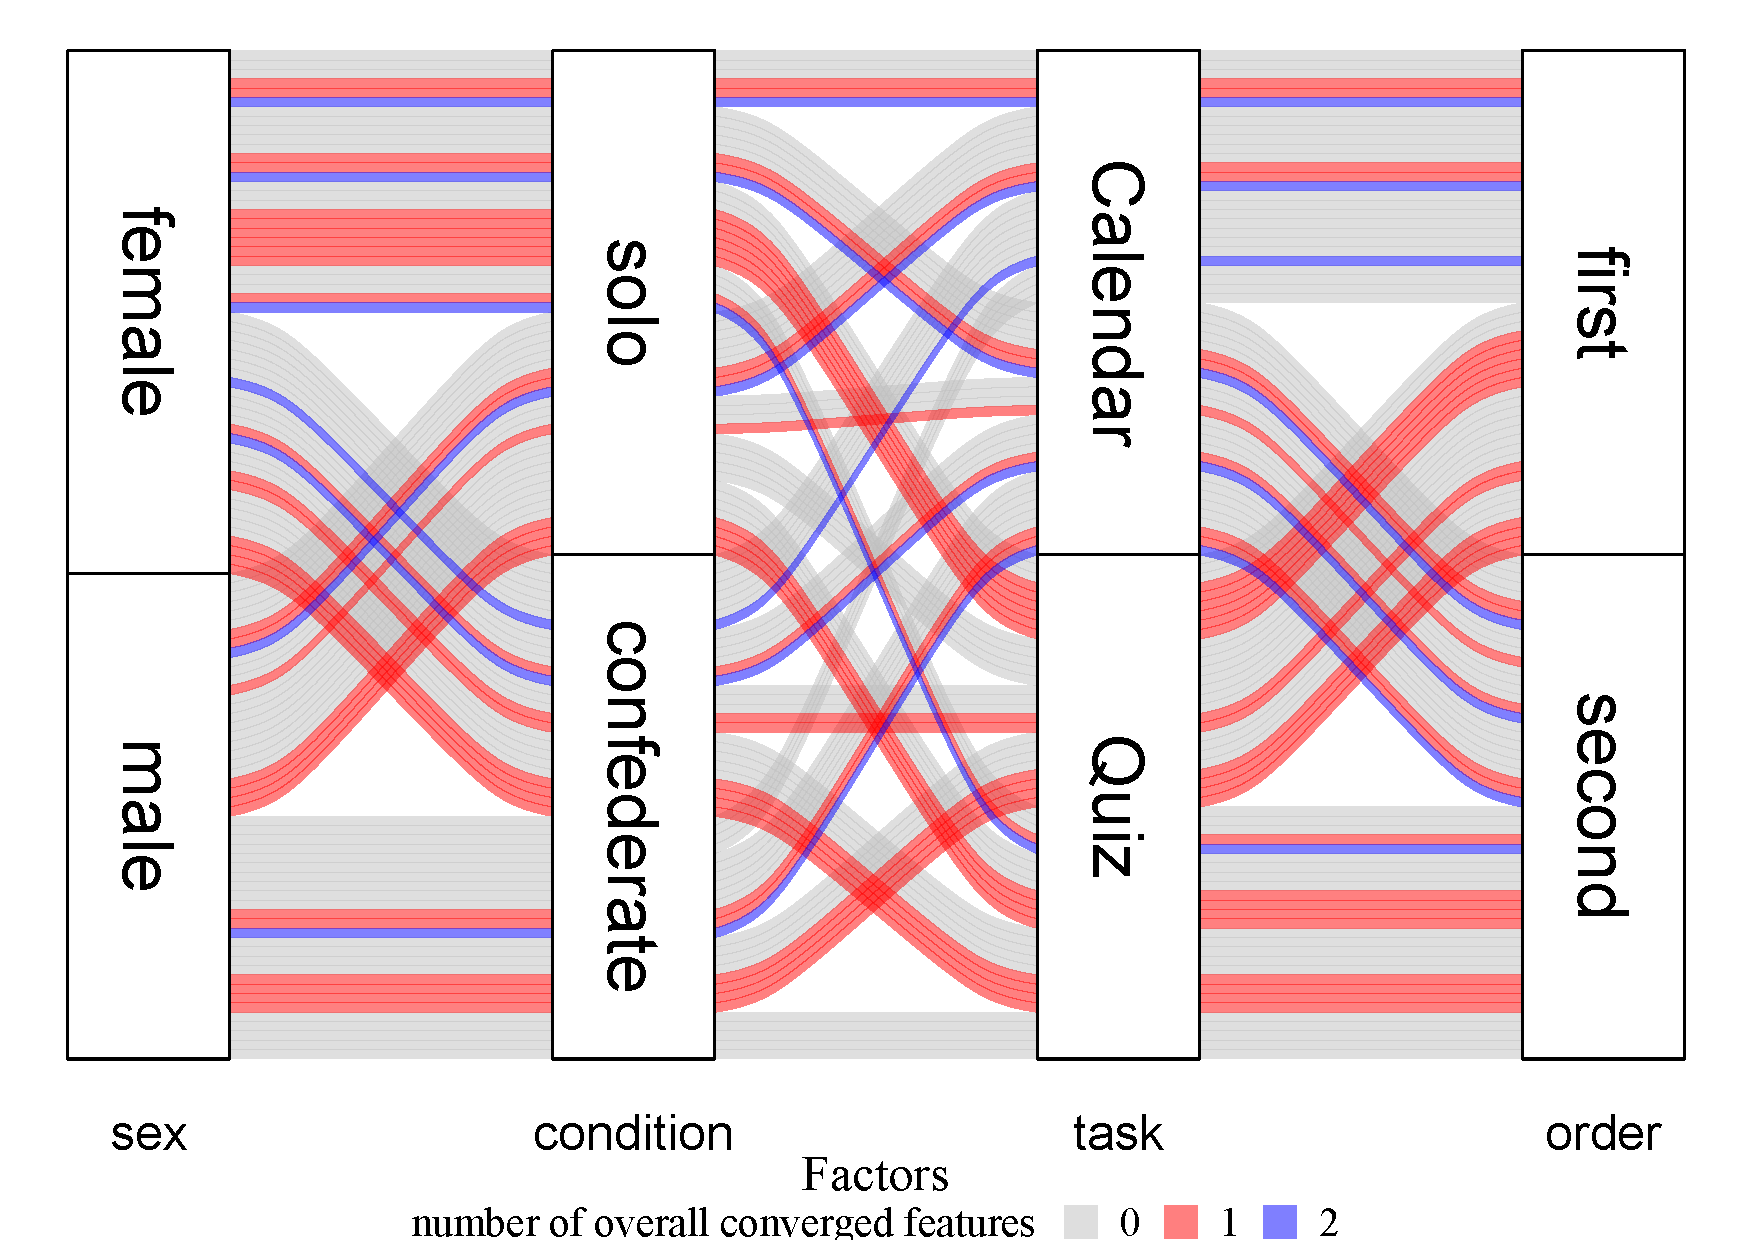
\includegraphics[width=\linewidth]{alluvial_4factors_numConv_strict}
	\caption
		[short caption]
		{Overview of the relation between the factors \emph{sex}, \emph{condition}, \emph{task}, and \emph{order} and the number of features that showed more convergence in total across the interactions.
		Each line represents one interaction.
		The \emph{sex} stratus refers to the sex of the participant, and the \emph{order} stratus to the position of an interaction in the order in which the task-condition combination was performed.
		The color of a line stands for the number of target features that showed overall convergence in this interaction, from none (zero features, in gray), through one (red), and up to two (blue).
		%		and up to all three features (green).
		For example, a blue line going through the strata sequence female $\rightarrow$ solo $\rightarrow$ Quiz $\rightarrow$ first represents an interaction with a female participant performing the Quiz task in solo condition first, where the participant converged in two out of the three target features.}
	\label{fig:alluvial}
\end{figure}

\section{Discussion and conclusion}
\label{sec:discussion_and_conclusion}

We have presented distributional and temporal analyses of differences in convergence of three vocal features in \ac{hci}, with emphasis on changes resulting from simultaneous, spoken \ac{hhi}.
The distributional analysis examined the difference in behavior of the features between interactions only with a computer-based device and interactions with both the device and a confederate, while the temporal analysis investigated the participants' account in the overall changes in proximity between the interlocutors.
To also consider the point in time during a session in which the confederate was speaking, the order factor was considered as well.
For all three features, it was found that
\begin{enumerate*}[(a)]
	\item the distributions differed more when the participant first interacted with the device alone, and
	\item more convergence was aggregated in the task that was performed first.
\end{enumerate*}
From these two findings, it can be concluded that chronological order of interactions affected the speech behavior of the participants.
Further analyses took the factors \emph{sex} and \emph{task} into account and indicated that female participants showed less convergence than male participants, but the task performed did not play any role in increasing the amount of convergence.
%Furthermore, as the task differ in their complexity and formality, this influences the convergence as well.
%The Calendar task is very formal and strict and thus the participants could use a very limited number of variability in their formulation.
%Furthermore, the role of the confederate speaker was similar to the role of Alexa, both had to give the same type of answers to the participant.
%Therefore, the presence of the confederate speaker does not influence the participants' speaking behavior that much.
%In the Quiz on the other hand, the participant and the confederate speaker build a team.
%Thus, their interaction is much more informal than the interaction with Alexa, which has the sole purpose of answering the questions.

The first speech input a participant encounters may cause a priming effect that, together with the natural tendency to converge to an interlocutor, results in more change in interactions that occur first.
However, the interchangeability of input (here, both \ac{hhi} and \ac{hci}) seems to hinder the ability of the participants to converge to Alexa.
One explanation for this may be that it is more natural for humans to accommodate to other humans, so once another human is involved, the accommodation towards the computer interlocutor is neglected.
Another possible explanation is that due to the multiple interlocutors, the participants do not have a steady target towards which to accommodate, which leads to a weakened convergence effect.
This is confirmed by the higher rate of convergence in the solo condition compared to the confederate condition.
Since \ac{hci} still lacks the mutuality of a comprehensive accommodation effect, the question arises whether these tendencies would be stronger in interactions with a single human versus interactions with two different human speakers simultaneously.
The higher number of convergence instances by females may be ascribed to the \ac{va} using a voice of the same sex and could be further investigated by using a \ac{va} with a male voice.

\section{Speaker roles and influences in sales calls}
\label{sec:speaker_roles_and_influences_in_sales_calls}

\subsection{\Acl{crqa}}
\label{subsec:crqa}

\Acf{crqa}\ldots

\section{abstract}

\section{Introduction}
\label{sec:introduction}

Sales leaders have always aimed to reason why some of their representatives -- henceforth \emph{reps} or \emph{\acp{ae}} -- consistently attain or exceed their goals and others do not \citep{Kovac2017its}.
Yet, sales executives rely on data that is inherently flawed, as it is based on reports from sources such as \ac{crm} systems, leaving executives in the dark about the happenings at the front lines.
As a result, the reasons for losing or winning a deal often remain a riddle, making sales an art based on anecdotes rather than science \citep{Yohn2016best, Martin2017six}.
In his seminal book, \citet{Gladwell2006tipping} writes, \textquote[pp.\ 83]{Part of what it means to have a persuasive personality is that you can draw others into your own rhythms and dictate the terms of the interaction}.
Supporting that, \citet{Orlob2018nine} found that star reps can make the prospect increase their speaking rate to match theirs, bringing the two sides closer with respect to this phonetic feature.

In this study, we focus on another phonetic feature, \ac{f0}.
This feature can also be interpreted and explained by people with little or no phonetic training, like \acp{ae}.
Furthermore, it can be easily controlled by speakers, making it a tangible tool for the \acp{ae} to exploit and improve their performance, as opposed to, e.g., more complex, acoustic features like \acp{mfcc} or changes in the \ac{ltas} that are often used in phonetic accommodation studies \citep{Levitan2011measuring,Borrie2019syncing}.

We use a large-scale corpus of real-world conversation, which takes the examination of phonetic accommodation out of the controlled, supervised experimental environment.
The conversations in the corpus are therefore more free-structured and flexible, as there are no instructions or defined tasks to perform, and presumably more authentic, since the interlocutors are driven solely by their own motivation to succeed and do not fill a temporary role as part of an experiment.

\Ac{crqa} \citep{Zbilut1998detecting}, a bivariate correlation technique, is used for the analysis (see \cref{subsec:crqa}).
This method finds instances where coordinates of two time series occur close to each other in some phase-space within a given radius.
Since \ac{crqa} can evaluate the degree to which the similarity of two time series changes over time, and can also determine the leading relationship between them, we find it suitable and informative for analyzing phonetic accommodation between two speakers.
A comprehensive overview of this method is presented by \citet{Wallot2018analyzing}, and the way it is used here is explained in \cref{subsec:crqa}.

The contribution of this work is therefore both in the methodology of measuring accommodation, and applying it in a practical situation.

%We hypothesize that since the prospect has agreed to meet for a demo and, in most cases, already heard about the proposed solution, the outcome of the call depends less on the prospect external condition and more on the personality of the sales person and her ability to build trust in the prospect.
%\todo{refer to where explain about dataset to justify the hypothesis.}

\subsection{Phonetic accommodation}
\label{subsec:phonetic_accommodation}

Depending on the situation, \ac{hhi} involves different levels of communication modality, such as facial expression, hand gestures, eye gaze, etc.
In this study, we concentrate on the phonetic level, as it is the main modality used in the sales calls dataset we analyze (see \cref{sec:dataset}).
It has been shown in various studies based on \ac{cat} \citep{Giles1991CAT,Gallois2015CAT} that humans naturally tend to change their speech behavior within a conversation based on the speech they hear from another human speaker \citep{Bailly2010speech,Babel2014novelty}.
Such mutual adjustment in \ac{hhi} also increases the success of the conversation \citep{Pickering2004toward} and affects the social distance between speakers \citep{Schweitzer2017social}.

The conversations in the large-scale corpus used here have an inherent structure and are longer than in typical experimental setups.
This encourages the use of \ac{crqa} to quantify the accommodation over the course of whole conversations to detect long-term relations and accommodation structures, instead of comparing two halves of the conversation or neighboring turns, as often done \citep{Levitan2013entrainment,Rahimi2018weighting}.

%Following that, we hypothesized that successful sales calls would show more distinct speech patterns and vocal accommodation behaviors than unsuccessful calls.

\subsection{Inside sales}
\label{subsec:inside_sales}

In recent years, many companies have adopted the concept of \emph{inside sales}, where \ac{b2b} sales are
done using web-based conferencing solutions, as opposed to face-to-face meetings with the clients.
Recent technological advancements allow automatic recording and transcription of inside sales calls, aggregating large-scale datasets.
These datasets include the audio of the calls and sometimes annotations such as the call success or the rating of the \ac{ae}.

Inside sales deals have a typical process:
first, a \ac{sdr} reaches out to a potential client (the \emph{prospect}) who has expressed interest in the company's product, which creates a \emph{lead}.
Subsequently, the \ac{sdr} shares basic details about the product and how it can help the prospect.
Finally, if the \ac{sdr} has managed to elicit initial interest, the lead turns into an \emph{opportunity}, and a demo call with a sales representative is scheduled.
Such demo calls are typically done using a web conferencing tool, such as Zoom\footnote{\url{https://zoom.us}} or GoToMeeting\footnote{\url{https://www.gotomeeting.com}}, which allows both sides to share their webcam and screen.

A relatively small dataset of such calls is analyzed in this work.
Since these calls were made as a first step after the prospect expressed interest in the company's product, it can be assumed that the behavior and verbal skills of the \ac{ae} will have a  larger weight in the success of the call than in calls that may fail solely because the product is of no interest to the prospect.

\section{Dataset}
\label{sec:dataset}

In this study we focus on calls of a single company.
The corpus for this study comprises only calls from an early stage of the sales opportunity that is also the first encounter between the participating \ac{ae} and the prospect.
Thus, these calls often include a description by the prospect of her business' history, challenges and plans, followed by a demo by the sales person that attempts to relate to those topics.
It is also important to note that although the \acp{ae} prepare for such calls, they are still spontaneous and in no way scripted.
With such set of calls, we can identify behavior patterns that are not related to the history between the two interlocutors or the content of previous conversations between them.
In some cases the prospect have already talked to an \ac{sdr} and/or communicated by email with the sales person.
However, to the best of our knowledge, this is the first voice call with the prospect.

The calls in this dataset were conducted using the Zoom platform, and were recorded automatically -- without any intervention from either side -- by Gong.io's system, which provides conversation intelligence services to said company.
Participants were notified of the recording, in compliance with relevant laws.
%The calls were then transcribed and diarized using an internal \ac{asr} system.

A single \ac{ae} and a single prospect participated in each call.
In total, 708 calls were used for analyses, each with a different customer company, with a total length of \SI{442}{\hour} (mean \SI{37.5}{\minute}, \ac{sd} \SI{15}{\minute}).
All of the calls are longer than 15 minutes, as many of the shorter calls were unsuccessful connection attempts.
Call recording started immediately following the first utterance by the prospect, and stopped when the meeting owner terminated it.
%This eliminates most issues related to one party waiting for the other party to join, and keeps only segments where both parties are present.
26 \acp{ae} (12 female) participated in the calls.
The vast majority of speakers on both sides were native speakers of American English.

We define a call as successful when a follow-up call under a more advanced stage is initiated or when an advancement in the opportunity is marked within one month.
Based on this criterion, 51 calls (\SI{7.2}{\percent}) were defined as successful, which is within the industry standard ratio for this kind of calls.
The average length of a failed call is \SI{37}{\minute} (\ac{sd} 15) and of a successful call, \SI{42}{\minute} (\ac{sd} 16.5).
A two-sample Wilcoxon test \cite{Wilcoxon1945individual} between failed and successful call duration yields a p-value of 0.04 with confidence level of \SI{95}{\percent}.
%Obviously, the labels of both criteria are noisy, as sales opportunities might be lost because of parameters more related to the fit between the offered product and the prospect's needs, the available budget of the prospect, the presence of competitors, legal issues that tamper the deal etc.

%We filtered out calls done by company personnel that are not sales people (for example, calls with \acp{sdr} that attempt to schedule demo meetings, or with Customer Success Managers who are often in charge of accompanying accounts after purchase).
%Sales people talked for X-X\% of the call (mean X\%, \ac{sd} X\%).
%The average duration of a monologue was X minutes and X seconds (\ac{sd} X minutes and X seconds) for sales people and prospect, respectively.
%The longest monologue of each participant in each call had a mean of X minutes and X seconds (\ac{sd} X and X seconds) for sales people and prospect, respectively.
%Automatic detection of questions based on the transcribed text showed that on average, the sales person asked X questions per minute (\ac{sd} X) compared with X (\ac{sd} X) for the prospect.
%We hypothesized that successful calls would show distinct patterns of phonetic convergence relative to unsuccessful calls.
%We measured the success of a call using two methods: (1) Based on the final outcome of the sales opportunity, being either won or lost.
%We call this method the "marriage" criterion, since it's similar to assessing a romantic date between two individuals as successful if it led to marriage and unsuccessful otherwise.

\section{Method}
\label{sec:method}

\subsection{Feature extraction}
\label{subsec:feature_extraction}

To increase temporal resolution, the audio signals were split into two-second slices.
Such fine-grained extraction makes the use of \ac{crqa} more elaborate, as it has more data points to consider (see \cref{subsec:crqa}).
Splitting the turns also creates equal, consecutive, and more comparable time units for an interaction without introducing artificial boundaries by dividing it into a predefined number of parts.
The slicing was done per turn, so that a slice contains only the speech of a single speaker.
Any remainder of a turn got a slice of its own.
When a speaker is not speaking (e.g., during the turn of the other interlocutor), it is assumed that the last produced value is maintained until the speech is renewed and a new value can be measured.
This way, no discontinuities are created and the same number of data points is extracted for both speakers, which creates a better temporal representation of the conversation.

Feature extraction was done sequentially for all the conversations using Praat\footnote{version 6.0.35} \citep{Boersma2001praat} scripts that first extracted the \ac{f0} value from the middle of each slice and then post-processed the output to acquire cleaner measures.

\subsection{\Acl{crqa}}
\label{subsec:crqa}

\begin{figure}[t]
	\centering
	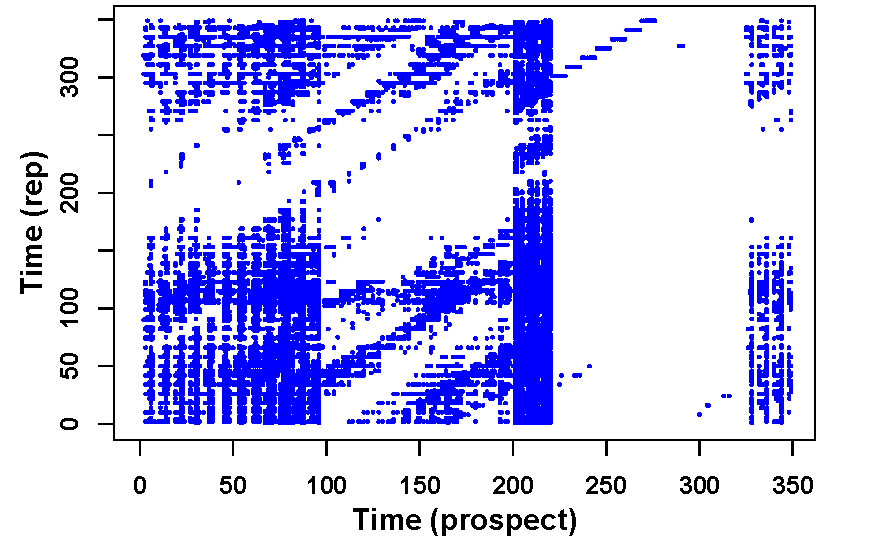
\includegraphics[width=\linewidth]{crqa_plot_115993376241473405}
	\caption
		[\acs{crqa} analysis of pitch in a sales call]
		{A recurrence plot generated for one of the analyzed conversations.
		The y-axis marks the conversation timeline, in time stamp, of the \ac{ae}, and the x-axis of the prospect.
		Each blue dot represents a co-visitation of a similar state.
		Blue dots forming an horizontal line indicate sustained recurrence between the two speakers (see \cref{sec:results} for details).
		Note that the time stamps on the axes are not the slices, but the embedded call time. 
		For example, the horizontal structures between time stamps 100 and 200 of the x-axis show such lasting recurrence.
		Horizontal lines above the \acl{los} (\acs{los}; the central horizontal line) indicate that the speaker on the y-axis leads the x-axis, and vice versa for lines below the \ac{los}.
		The blank area between time stamps 220 and 330 of the x-axis point to a portion of the call where the speakers were more distant from each other.}
	\label{fig:crqa_plot}
	\todo[inline]{make the plot square, to make it clearer that the times have the same length}
\end{figure}

We treat the measured value sequences of the extracted features from the speakers as two non-seasonal time series and use \acf{crqa} to detect convergence between them.
\Ac{crqa} is an extension of recurrence quantification analysis \citep{Webber2005recurrence}, but with recurrence quantification of two different time series rather than a single one.
As such, \ac{crqa} is a quantification technique for non-linear dynamical systems that describes when and to what extent two time series visit similar states, or \emph{recurrences} (also called co-visitations) over the course of an interaction.
Due to its ability to detect these similarities non-linearly, \ac{crqa} can be utilized to measure accommodation in the scope of entire conversations rather than taking only neighboring turns into account \citep{Levitan2013entrainment}.
For example, it has already been used to describe behavior in conversations \citep{Duran2017conversing} and to measure conversational entrainment for assessing speech pathology \citep{Borrie2019syncing}.
A recurrence plot can be generated to visualize the relationships of the co-visitations.
\cref{fig:crqa_plot} shows such a plot.
See \cref{sec:results} for details regarding the output values of \ac{crqa}.

\Ac{crqa} requires three parameters to run: \emph{delay}, \emph{embedding dimensions}, and \emph{radius}.
\emph{Delay} estimates the temporal shift required to make the two time series maximally aligned.
It is measured by the same time unit as the time series, in this study, a slice (see \cref{subsec:feature_extraction}).
\emph{Embedding dimensions} are the number of dimensions into which the data points are embedded.
These dimensions are delayed copies of the original time series $S(t)$ created by adding a lag $k$ to them.
Typically, multiple lags are considered, which create the dimensions of embedding $S(t + nk)$.
\emph{Radius} determines the margin within which two data points are considered a recurrent instance.
Distances between the data points are measured in the embedded space defined by embedding dimensions, using the same unit used for measuring the values of the time series.
These parameters are a key aspect in \ac{crqa} and how they are set is crucial for its outcome.
Although some best-practice guidelines are suggested by \citet{Coco2014crqa-r}, there is no standard way for optimizing these parameters, especially due to the fact that they depend on the nature and characteristics of the data.

We therefore utilized a method similar to the one presented by \citet{Marwan2007recurrence}.
The delay parameter was determined by finding the lag that minimizes the mutual information between the two time series.
This provides a delay that is not too short to miss the different distributions, but also not too long to lose the dependency between the time series.
The lag with the \emph{minimal} mutual information was selected, regardless of where it started to level off.
Then, the number of embedding dimensions was obtained using false nearest neighbors \citep{Kennel1992determining}.
This algorithm determines the minimum embedding dimension necessary to reconstruct the state space of a dynamical system with time delay embedding \citep{Abarbanel1993local}.
We used a neighborhood diameter equal to the standard deviation of the time series and set a limit of 20 embedding dimensions (which was never reached).
Finally, the radius was calculated in two steps.
First, the goal \ac{rr} and a list of potential radii were set.
We set the goal \ac{rr} to \SI{10}{\percent}, which is relatively high (e.g., compared to the \SIrange{2}{5}{\percent} of \citet{Coco2014crqa-r}).
Setting the goal \ac{rr} to a higher value results in a stricter optimization that will reward closer recurrences in the analysis.
The potential radii were generated by evenly spreading 20 candidates from 0 to the maximum value that occurs in the times series.
After that, each radius, along withe already optimized delay and embedding dimensions, was used to perform a \ac{crqa}.
This step also introduced a stricter policy, as only horizontal lines longer than \SI{1}{\percent} of the length of the time series were counted, as opposed to the typical setup that considers all horizontal lines.
With an average length of \SI{37.5}{minutes}, this means that lines longer than 11 time units, compared to the a typical setup with the minimal length of two time units (e.g., as done by \citet{Borrie2019syncing}).
This ensured that only long-term recurrences were taken into account, and filtered out shorter, possibly more random effects.
% note: calculated by multiplying 37.5 minutes * 60 to get seconds. then divide by 2 since each time unit is 2 seconds and again divide by 100 to get one percent of it.
Finally, the radius that results in the smallest absolute distance from the goal \ac{rr} was taken as the optimized radius to use for the \ac{crqa}.
The entire optimization process was done for each call separately.

\section{Results}
\label{sec:results}

%In total, 708 calls were analyzed, from which 51 (\SI{7.2}{\percent}) were marked as successful as per the definition explained in \cref{sec:dataset}, which is an expected ratio in this kind of calls.
The \ac{crqa} yields 7 output values for each conversation:

\begin{description}[wide, nosep]
	\item[\Acf{rr}] the percentage of recurrent values between the two time series out of all the values.
	\item[Percentage determinism (DET)] the percentage of recurrences forming diagonal lines (with the minimum length being \SI{1}{\percent} of the series length).
	\item[number of lines (NRLINE)] The total number of lines formed by the recurrent values, i.e., the amount of accommodation between the two speakers that lasts longer than \SI{1}{\percent} of the time.
	Also referred to as \emph{sustained recurrence} by \citet{Borrie2019syncing}.
	\item[Maximal length (maxL)] the longest time period of recurrence, i.e., the longest time the speakers' speech remained close.
	\item[Average length (L)] the average time of recurrence.
	\item[Entropy (ENTR)] Shannon information entropy of diagonal line lengths longer than the minimum length.
	Describes the variability of the amount of accommodation between the two speakers across the whole call.
	\item[Normalized entropy (rENTR)] the entropy normalized by the number of lines formed by the recurrent values.
	This measure gives an idea how the speakers vary across multiple calls with different properties.
\end{description}

Since we compare multiple variables, Bonferroni correction was applied, so that the overall error rate across all variables is \num{0.05}.
Therefore, for a single comparison to be significant, it must be lower than $\alpha = 0.007$.
The non-parametric two-sample Wilcoxon test \citep{Wilcoxon1945individual} was used to determine the significance levels.
\cref{tab:crqa_results} shows a summary of means and p-values of these outputs between failed and successful calls.
The \ac{rr} mean value is about 10 in all groups, which proves to be a suitable goal for optimizing the parameters (see \cref{subsec:crqa}).
Significant differences between failed and successful calls were found for the values DET, NRLINE, and rENTR.
The first two, along with their higher means for the failed calls, indicate more time-synchronized convergence in the failed calls.
The latter is harder to interpret, especially due to the similar means for successful and failed calls.
It therefore seems that the behavior in both cases is evenly predicted, but differently across calls.
One possible factor influencing these behaviors is related to the interlocutor leading the convergence, rather than the fact that it occurs at all.

\begin{table}[t]
	\caption{P-values of the two-sample Wilcoxon test comparing the \ac{crqa} output values between calls with success/fail outcome and their respective mean values.
		Significant values based on the adjusted p-value are set in bold.}
	\label{tab:crqa_results}
	\begin{tabularx}{\linewidth}{XSSSS}
		\toprule
		& {\thead{\acs{rr}}} & {\thead{DET}} & {\thead{NRLINE}}	& {\thead{maxL}} \\
		\midrule
		p 				& 0.9		& \bfseries $\ll$ 0.001	& \bfseries $\ll$ 0.001	& 0.7  \\
		mean success	& 10.1		& 2.2					& 84.0					& 31.3 \\
		mean fail		& 10.0		& 5.9					& 174.0					& 32.9 \\
		
		%			p (leaders)		& 0.7		& 0.1						& 0.05						& 0.18\\
		%			mean \acsp{ae}	& 10.0		& 6.1						& 186.7						& 35.2\\
		%			mean prospect	& 10.1		& 5.4						& 154.4						& 31.2\\
		\midrule
		& {\thead{L}} 	& {\thead{ENTR}} 	& {\thead{rENTR}} 	& 						\\
		\midrule
		p 				& 0.07				& 0.1				& \bfseries 0.0058	& 	\\
		mean success	& 17.8				& 1.4				& 0.8				& 	\\
		mean fail		& 15.3				& 1.5				& 0.8				& 	\\
		
		%			p (leaders)		& 0.9		& 0.07		& 0.55					& {\qquad\qquad}\\
		%			mean \acsp{ae}	& 15.2		& 1.5		& 0.8					& {\qquad\qquad}\\
		%			mean prospect	& 15.7		& 1.4		& 0.8					& {\qquad\qquad}\\
		\bottomrule	
	\end{tabularx}
\end{table}

To shed more light on the role of a leading partner, we used \acl{cc} to determine which interlocutor leads the change in behavior.
As shown in \cref{fig:crqa_plot}, \ac{crqa} reports at which points in time the speakers were more inclined to be closer to each other.
As an extension, \acl{cc} finds the degree to which two time series are synchronized at different points in time.
For each such point, called \emph{lag}, the \acl{cc} function evaluates the correlation between the time series.
By iterating over a set of time points, the shift needed to make the time series maximally correlated can be found.
If this lag is positive, the first time series needs to be shifted forward to achieve maximal correlation, and vice versa.
In the context of convergence, \ac{cc} calculates the direction of the shift, which indicates which speaker leads the change.
The \acl{cc} function was not limited to a specific range of shifts, so that all possible lags were examined.
The lag associated with the maximal correlation -- and only it -- was used to determine the leader.
Since these calls have a typical structure, it is also interesting to see at which point of the conversation the maximal correlation occurs.
\cref{fig:barplot_conv_leaders} shows the time, in percentage, in which the maximal correlation occurred for \acp{ae} and prospects in successful and failed calls.
The difference between the lag position distribution of reps and prospects is significant, with a p-value of \num{0.0065} at $\alpha = 0.05$.
However, the differences between successful and failed calls within the leading speakers are not significant.
It is also evident that when the reps lead, they do so consistently at the very beginning of the conversation, all the more so in successful calls, whereas the prospects' lead varies much more and generally happens at a much later time.

\section{Discussion}
\label{discussion}

The results of the study show two sides of \ac{crqa} with respect to call success and role detection.

On the one hand, successful and failed calls could be distinguished by three of the \ac{crqa} output values.
Although based on \ac{hhi} studies it might be hypothesized that recurrence is more likely to occur in successful calls, the means of two of the three values suggest the opposite.
Surprisingly, this stands in line with some studies from sales research that show more \enquote{desperate} behavior from the rep side when a call seems to fail.
For example, over-emphasizing the deal's \ac{roi} -- with the hope that it will convince the prospect to buy -- often achieves the opposite effect \citep{Orlob2018roi}.
Another possible explanation is that reps give up their own lead in the call (see below) when a call is on the verge of failing, and instead let the prospect lead, either as a natural tendency or to give a better feeling.

On the other hand, utilizing \acl{cc} lags (i.e., how the recurrence needs to shift for the speakers to be maximally aligned) was useful for differentiating between the leader in the calls.
When \acp{ae} lead, they tend to do so at an earlier stage than prospects, especially in successful calls.
This, along with the \ac{crqa} results explained above, suggests that \acp{ae} do not necessarily always lead the conversation, but they know when to take advantage of it to improve their stance in calls.

Future research on this topic may go into three main directions.
First, deepening the aspect of the relationship between the \acp{ae} and the prospects by examining the mutual changes not only within single calls, but over the course of several meetings.
This could shed light on long-term changes and connect changes to the success of the deal.
Secondly, distinguishing between different \acp{ae} to find behaviors of sub-groups.
For example, sales persons with higher ratings (star reps) might be revealed to better exploit accommodation and trigger different behavior on the prospect side to increase their chance of closing a deal.
Lastly, different methods could be applied to predict the success of a call.
Specifically, machine learning methods that are good at capturing serial changes, such as recurrent neural networks, can be used to train such prediction models.
All of these direction can also be combined with more features to measure and more calls to analyze to reveal more consistent accommodation patterns.

\begin{figure}[t]
	\centering
	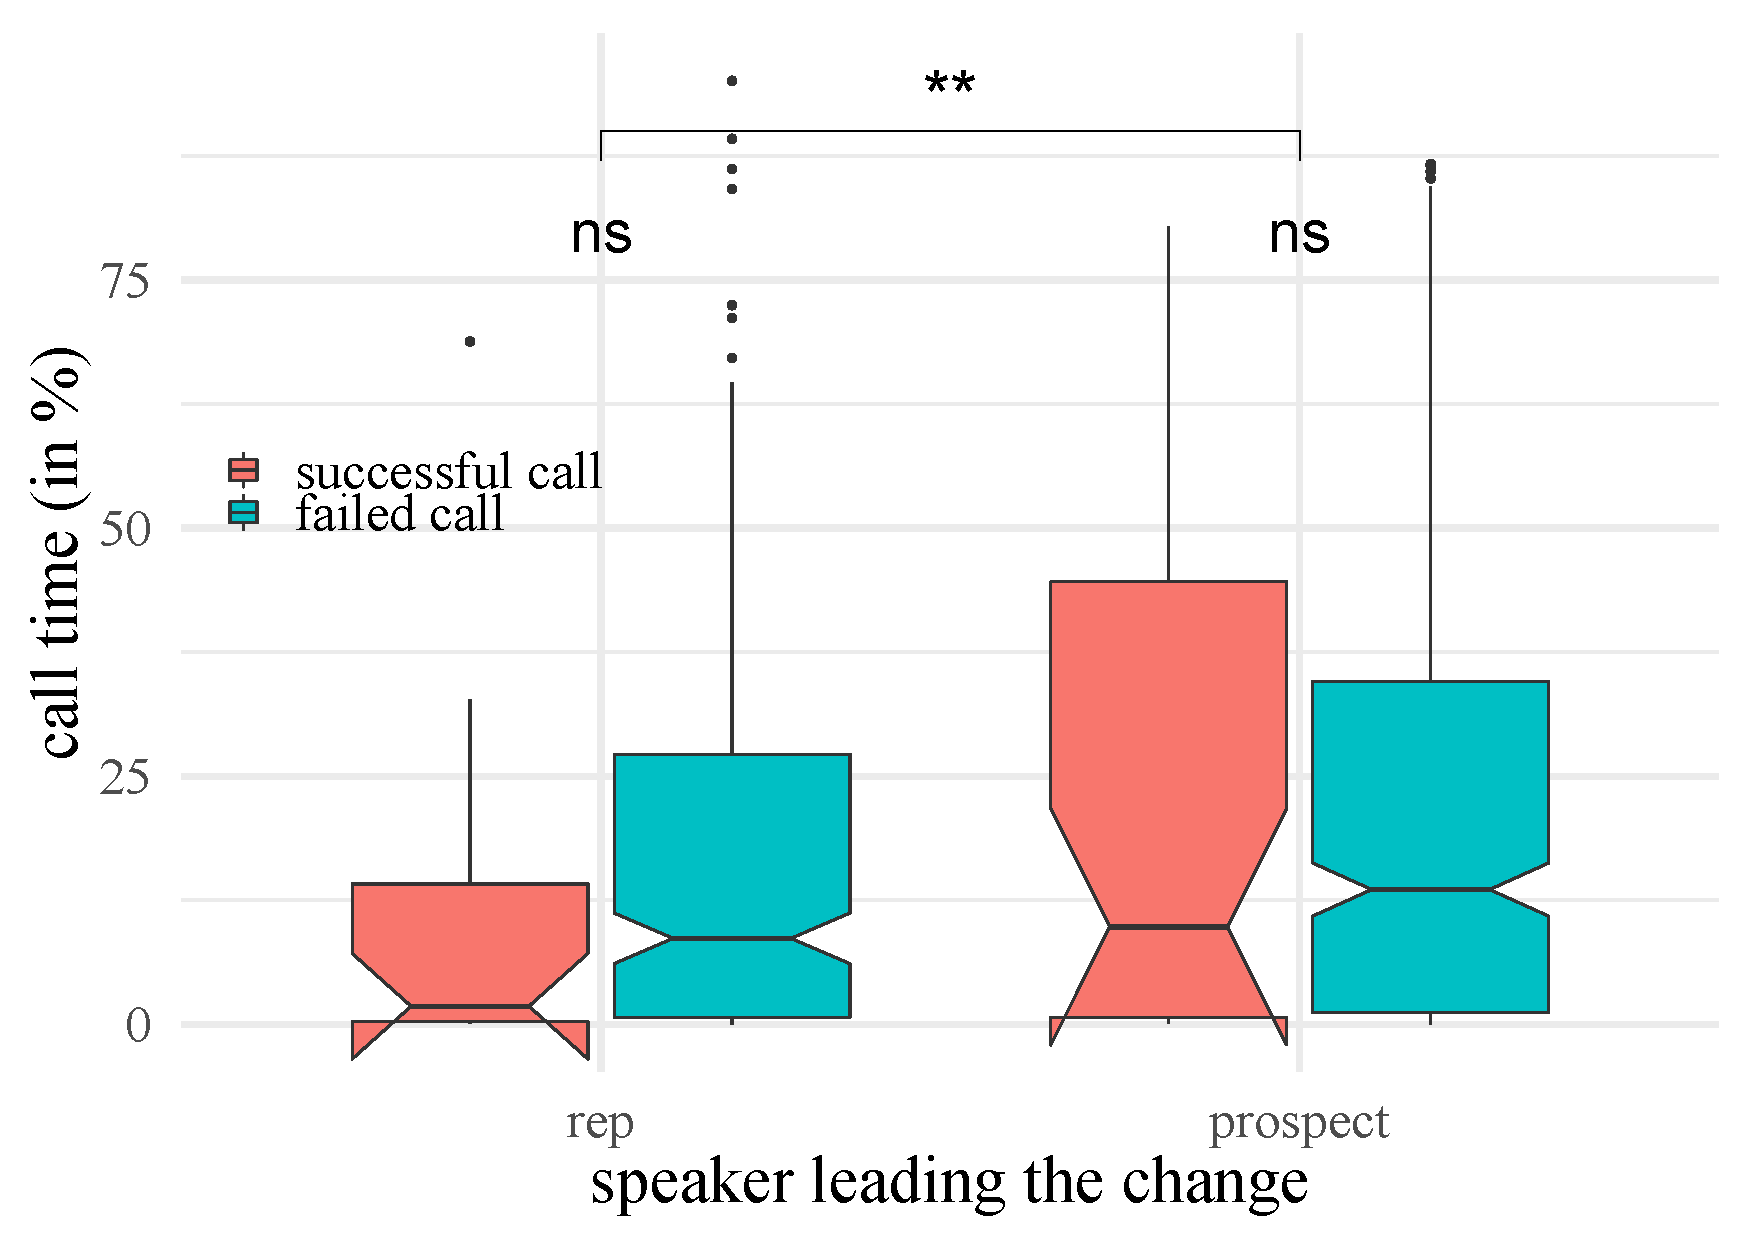
\includegraphics[width=\linewidth]{boxplot_ccf}
	\caption
		[Comparison between sales reps' and prospects' maximal \acl{cc} point in conversation for successful and failed calls.]
		{Comparison between the time of the call in which the maximal \acl{cc} occurs.
		The x-axis groups the calls based on the speaker, and the fill color further separates the calls to successful and failed ones.
		The y-axis points to the time in the call, in which the maximal correlation was detected.
		The horizontal lines within the boxes represent the median,
		%		the notches stand for the \SI{95}{\percent} confident level of the median, the area inside the boxes include the \acf{iqr} of values, the vertical lines outside the boxes show the value within the third quartile + 1.5~$\protect\cdot$~\ac{iqr}, and the isolated dots are the outliers.
		The significance level based on a Wilcoxon test comparing the two groups and their subgroups is given above the boxes.}
	\label{fig:barplot_conv_leaders}
	%	\todo[inline]{use logarithmic y-scale?}
\end{figure}


\section{Conclusion}
\label{sec:conclusion}

We have presented a study that examines phonetic accommodation in real-world sales calls.
The focus was on mutual proximity of \acl{f0} between sales persons and prospects to find both how close they are to each other in general across the call, and how quickly changes in proximity occur and by whom they are initiated.
This was done by \acf{crqa} and \aclp{cc}, which together provide various measures regarding recurrence between the speakers and who leads the other in terms of \acl{f0} changes.
A corpus of 708 calls was used for the analyses, which makes it possible to find more global, consistent effects that are not influenced by the design of a specific experimental setting.
The results show significant differences in some of the values between successful and failed calls, and significant differences between the leading behavior of sales persons and prospects.
These findings encourage further investigations, like looking for other predictors of successful calls and examining the influence of additional features and factors on the success of calls.

